\section{Performance}
\label{sec:performance}

We study the separation of the $\dihiggs$ signal from the $\ttbar$ background,
achieved by the LR $P(\vecy)$ given by Eq.~(\ref{eq:memLR}),
using samples of signal and background events produced by Monte Carlo (MC) simulation.
The samples are simulated at LO and at NLO accuracy in pQCD
and are analyzed at MC-truth as well as at detector level.
The LO and NLO $\dihiggs$ signal samples each contain about three hundred thousand events
and the LO and NLO $\ttbar$ background samples each contain about five million events.
All samples simulated at LO accuracy in pQCD are produced with the program $\textsc{MadGraph\_aMCatNLO}$ $2.2.2$,
while the samples simulated at NLO accuracy in pQCD are produced using the program $\textsc{POWHEG}$ $v2$~\cite{POWHEG1,POWHEG2,POWHEG3,POWHEGTTBAR1,POWHEGTTBAR2,POWHEGHH1,POWHEGHH2}.
The \textrm{NNPDF3.0} LO set of PDF is used for the simulation of the LO samples and the \textrm{NNPDF3.0} NLO set for the NLO samples~\cite{NNPDF1,NNPDF2,NNPDF3}.
Parton shower and hadronization processes are modeled using the program $\textsc{PYTHIA}$ $v8.2$~\cite{Sjostrand:2014zea} with the tune \textrm{CP5}~\cite{Sirunyan:2019dfx}.
All events are generated for proton-proton collisions at $\sqrt{s} = 13$~\TeV center-of-mass energy.
Events in which the electrons or muons originate from $\Pgt$ lepton decays,
\ie from the decay chains $\PW^{+} \to \Pgt^{+}\Pnu_{\Pgt} \to \Plepton^{+}\Pnu_{\Plepton}\APnu_{\Pgt}\Pnu_{\Pgt}$ or 
$\PW^{-} \to \Pgt^{-}\APnu_{\Pgt} \to \Plepton^{-}\APnu_{\Plepton}\Pnu_{\Pgt}\APnu_{\Pgt}$, are discarded.
Detector effects are simulated using the $\textsc{DELPHES}$ fast-simulation package~\cite{deFavereau:2013fsa} with the card for the CMS detector.
On average forty inelastic proton-proton interactions (pileup) are added to each simulated event
in order to simulate the data-taking conditions during Run $2$ of the LHC.

Jets are reconstructed using the anti-$\kt$ algorithm~\cite{Cacciari:2008gp, Cacciari:2011ma} with a distance parameter of $0.4$.
We produce two separate collections of jets for studying the performance of the MEM at MC-truth and at detector level,
using either all stable generator-level particles or the detector-level particle-flow objects created by $\textsc{DELPHES}$ as input to the jet reconstruction.
We refer to the first collection as generator-level and to the second as detector-level jets.
The generator-level jets exclude the particles from pileup.
The energy of jets reconstructed at detector level is corrected for pileup effects using the method described in Refs.~\cite{Cacciari:2008gn, Cacciari:2007fd}
and calibrated as function of jet $\pT$ and $\eta$.
The calibration is performed in two stages. 
In the first stage, the energy of detector-level jets is calibrated to match the energy of generator-level jets,
while in the second stage, the energy of generator-level jets is calibrated to match the energy of the bottom quarks that result from $\PHiggs$ boson or top quark decays at parton level.
The first stage of the jet energy calibration is applied to all detector-level jets, 
while the second stage is applied to the generator-level jets and to those detector-level jets that are tagged, on detector level, as originating from the hadronization of a bottom quark.
We refer to the latter jets as $\Pbottom$-jets.

The simulated $\dihiggs$ signal and $\ttbar$ background events considered in this section are required to pass event selection criteria,
which follow loosely the analysis of $\dihiggs$ production in the decay channel $\Pbottom\APbottom\PW\PW\virt$ performed by the CMS collaboration in LHC Run $2$~\cite{HIG-17-006}.
The events are required to contain exactly two isolated leptons, which must be within the region $\abs{\eta} < 2.5$ if they are electrons and $\abs{\eta} < 2.4$ if they are muons.
The isolation of the leptons is computed by summing the $\pT$ of detector-level particle-flow objects that are within a cone of size
$\delta R = \sqrt{(\delta\eta)^{2} + (\delta\phi)^{2}} = 0.5$ around the lepton direction, excluding the lepton itself.
The sum is corrected for the contribution of particles from pileup using the method described in Refs.~\cite{Cacciari:2008gn, Cacciari:2007fd}.
Leptons are considered isolated if the pileup-corrected sum amounts to less than $0.10$ times the $\pT$ of the lepton.
The lepton of higher $\pT$ is required to have $\pT > 25$~\GeV and the lepton of lower $\pT$ must have $\pT > 15$~\GeV.
The $\pT$ thresholds applied to the leptons are motivated by trigger requirements.
The events are further required to contain two jets of $\pT > 25$~\GeV and $\abs{\eta} < 2.4$ that are both tagged as $\Pbottom$-jets on detector level.
Events containing more than two $\Pbottom$-tagged jets of $\pT > 25$~\GeV and $\abs{\eta} < 2.4$ are vetoed.
The latter condition only rejects a negligible fraction of events, amounting to $X.X\%$ of the $\dihiggs$ signal and to $X.X\%$ of the $\ttbar$ background, 
and avoids ambiguities in choosing the pair of $\Pbottom$-jets 
when computing the weights $w_{0}(\vecy)$ and $w_{1}(\vecy)$ according to Eqs.~\ref{eq:mem_signal} and~\ref{eq:mem_background}.

Fig.~\ref{fig:mbb} shows the distribution in $\mbb$, the mass of the two $\Pbottom$-tagged jets at detector level, 
in $\dihiggs$ signal and $\ttbar$ background events that pass the selection criteria described in the previous paragraph.
Only events in which both detector-level jets are matched, within a cone of size $\delta R = 0.3$, 
to bottom quarks that originate from either $\PHiggs$ boson or from top quark decays, are shown in the figure.
According to the $\textsc{DELPHES}$ simulation, 
$XX.X\%$ of $\dihiggs$ and $XX.X\%$ of $\ttbar$ events that pass the selection criteria described in the previous paragraph fulfill this matching condition,
\ie in $X.X\%$ of selected $\dihiggs$ and $X.X\%$ of selected $\ttbar$ events one of the bottom quarks is not reconstructed as $\Pbottom$-jet at detector level
and a light quark or gluon jet is misidentified as $\Pbottom$-jet instead.
The figure shows that the jet calibration shifts the peak of the $\mbb$ distribution by about $20\%$.
After calibration, the $\mbb$ distribution in $\dihiggs$ signal events peaks close to $125$~\GeV.
The calibration also reduces the relative width, defined as the root mean square divided by the mean, of the $\mbb$ distribution in $\dihiggs$ signal events by about $20\%$.

\begin{figure}
\ifx\ver\verPreprint
\setlength{\unitlength}{1mm}
\begin{center}
\begin{picture}(160,67)(0,0)
\put(-1.0, 1.0){\mbox{\includegraphics*[height=66mm]
 {plots/mbb_calibrated_vs_uncalibrated_signal.pdf}}}
\put(80.0, 0.0){\mbox{\includegraphics*[height=67mm]
 {plots/mbb_calibrated_vs_uncalibrated_background.pdf}}}
\end{picture}
\end{center}
\fi
\ifx\ver\verPAPER
\centering
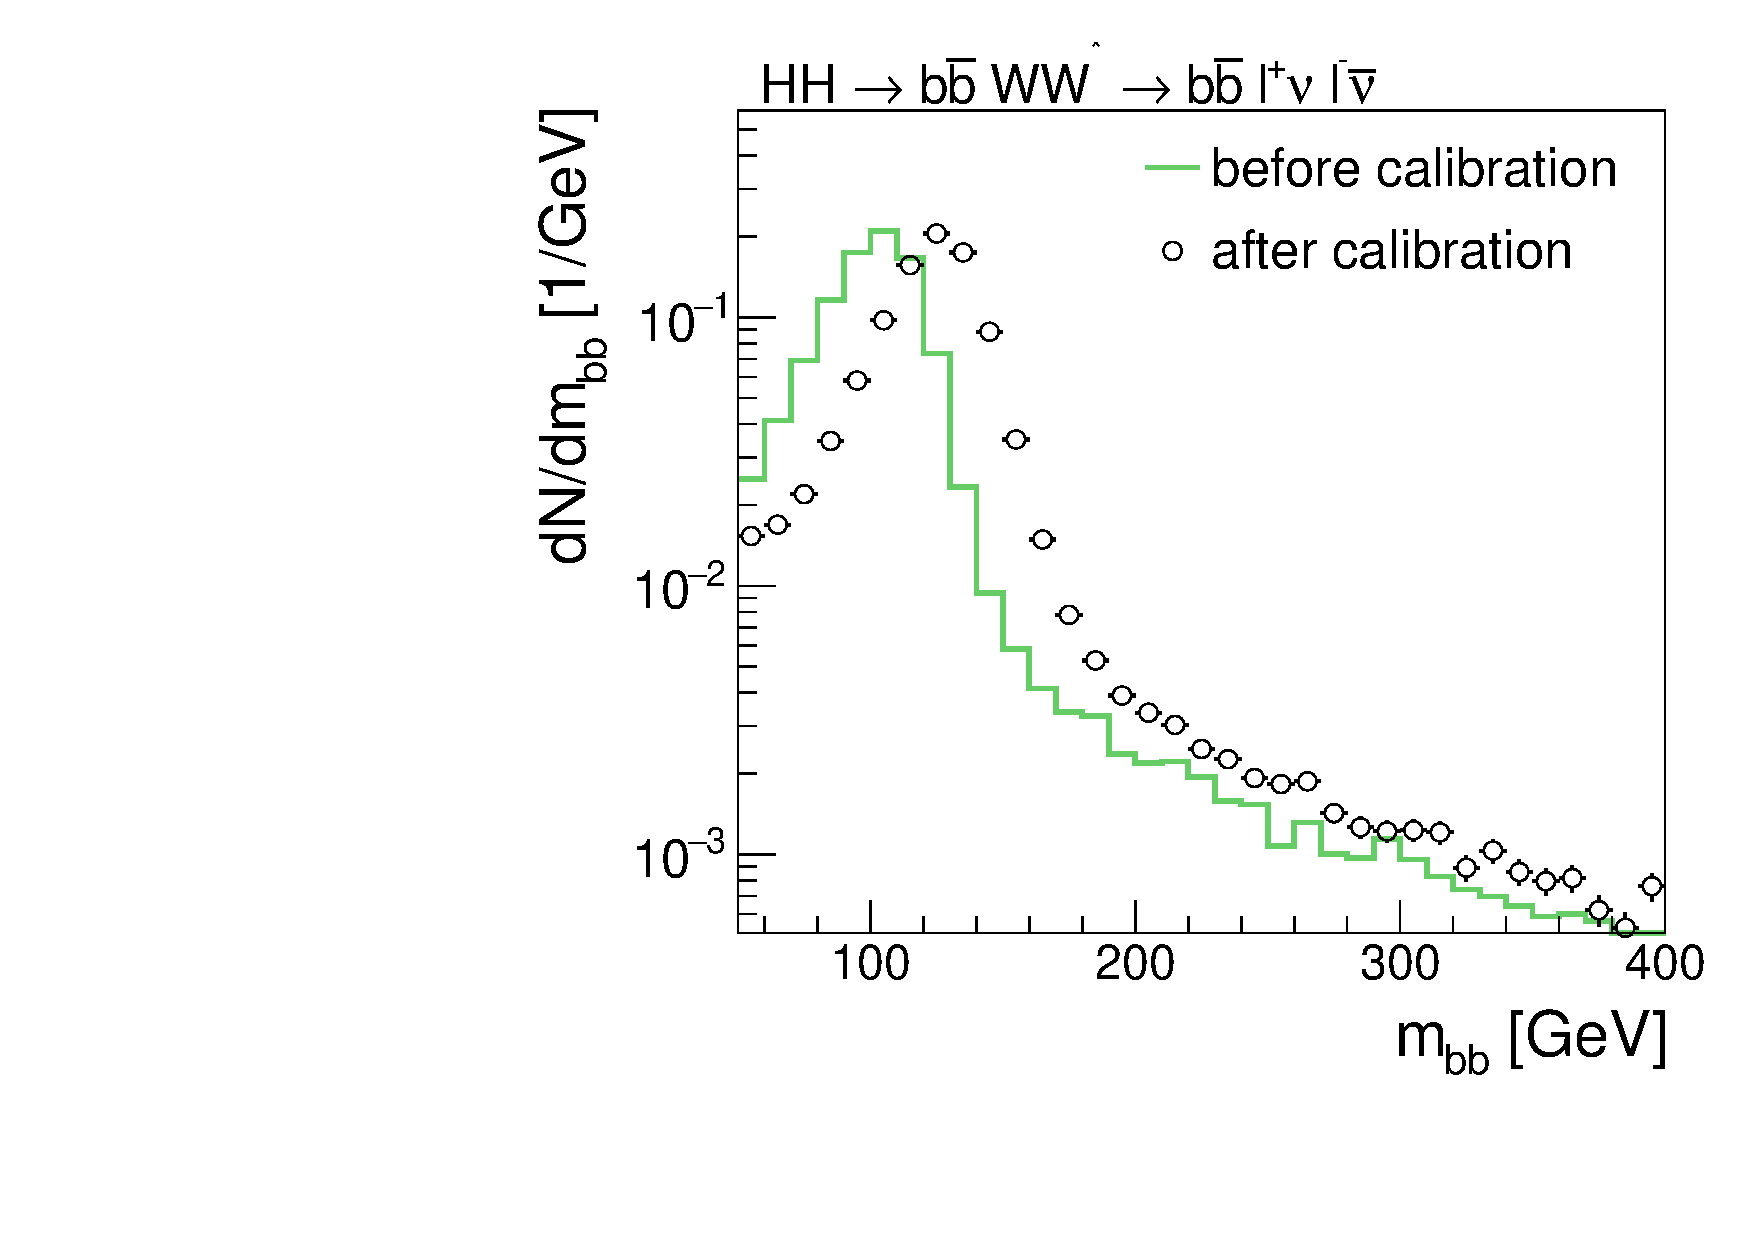
\includegraphics[width=0.48\textwidth]{plots/mbb_calibrated_vs_uncalibrated_signal.pdf}
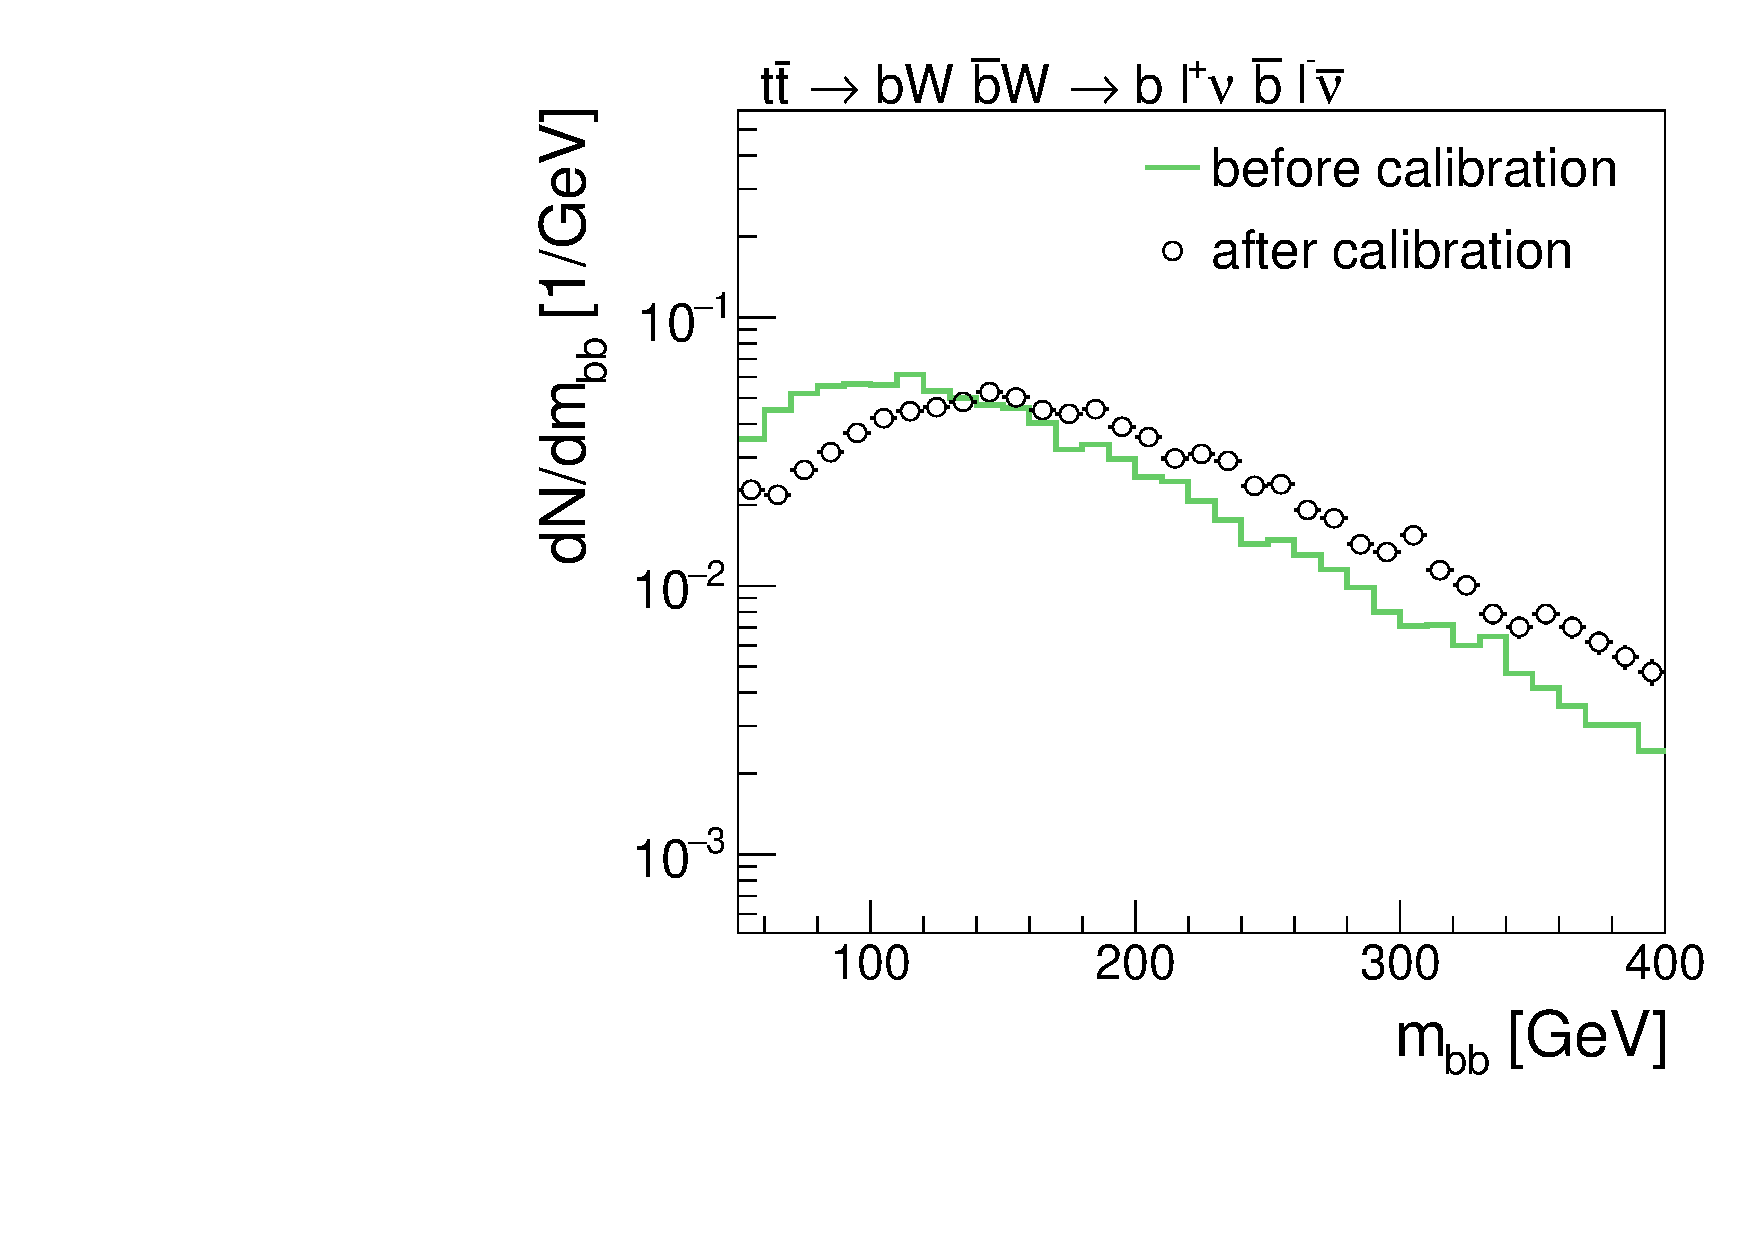
\includegraphics[width=0.48\textwidth]{plots/mbb_calibrated_vs_uncalibrated_background.pdf}
\fi
\caption{
  Distribution in $\mbb$, the mass of the two detector-level jets that are tagged as $\Pbottom$-jets,
  in $\dihiggs$ signal (left) and $\ttbar$ background (right) events before and after the jet energy calibration is applied.
}
\label{fig:mbb}
\end{figure}


